\documentclass{beamer}

\usepackage[italian]{babel}
\usepackage[T1]{fontenc}
\usepackage{beamerthemeAntibes}
\usepackage{graphicx}
\usepackage{listings}
\usepackage[utf8]{inputenc} 
\usepackage{epsfig}  
\usepackage{amsmath} 
\usepackage{multicol}
\usepackage{amsfonts}
\usepackage{hyperref}
\usepackage{listings}
\usepackage{changepage}

\lstset{
  basicstyle=\footnotesize,
  language=C,                % choose the language of the code                 % where to put the line-numbers
  backgroundcolor=\color{white},  % choose the background color. You must add \usepackage{color}
  showspaces=false,               % show spaces adding particular underscores
  showstringspaces=false,         % underline spaces within strings
  showtabs=false,                 % show tabs within strings adding particular underscores
  tabsize=2,                      % sets default tabsize to 2 spaces
  captionpos=b,                   % sets the caption-position to bottom
  breaklines=true,                % sets automatic line breaking
  breakatwhitespace=true,         % sets if automatic breaks should only happen at whitespace
  title=\lstname,                 % show the filename of files included with \lstinputlisting;
}



\setbeamertemplate{itemize/enumerate body begin}{\footnotesize}

\title{Social Networks}
\author{Luigi Giugliano$^1$, Steven Rosario Sirchia$^1$}
\institute{$^1$Università degli studi di Salerno}


\begin{document}

\begin{frame}
   \maketitle
\end{frame}

\begin{frame}
\frametitle{Introduction}
The purpose of our work is to test different algorithms in the three fundamental areas for assembling any search engine offering a Sponsored Search system:
\begin{itemize}
\item \textbf{Ranking} of web documents
\item \textbf{Matching} of words inside documents
\item \textbf{Auctions} for acquiring advertisement slots.
\end{itemize}
We will briefly talk about the proposed algorithms, and then compare running times and results obtained from their execution more in detail, suggesting what combination of algorithms seems to be the best for realizing a new search engine.
\end{frame}

\begin{frame}
  \frametitle{Overview}
  \footnotesize \tableofcontents
\end{frame}

\AtBeginSection[]
  {
     \begin{frame}<beamer>
     \frametitle{Overview}
   \footnotesize \tableofcontents[currentsection]
     \end{frame}
}

\section{Ranking}
\subsection{Page Rank}
\begin{frame}
\frametitle{Page Rank}
\begin{block}{Page Rank}
The intuition behind \emph{Page Rank} is:
\center``a page is important if it is cited by other important pages''.
\end{block}
This intuition rises from the usual endorsement mode, for example, among academic or governmental pages, among bloggers, or among personal pages more generally. It is also the dominant mode in the scientific literature.
\end{frame}

\begin{frame}
\frametitle{Algorithm}
We can think of PageRank as a kind of “fluid” that circulates through the network, passing from node to node across edges, and pooling at the nodes that are the most important.
\center
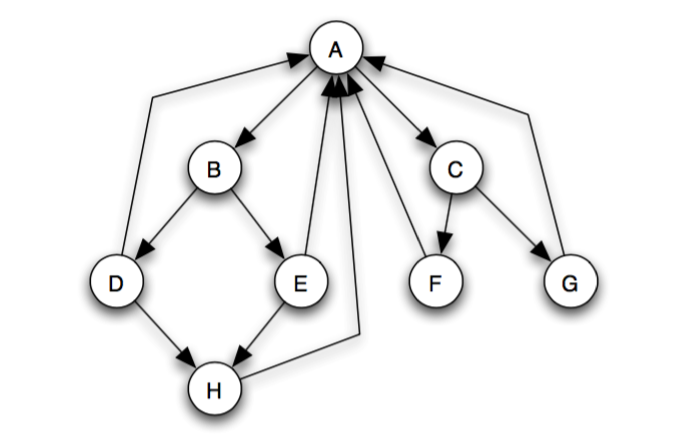
\includegraphics[scale=0.3]{img/general_network.png} 
\end{frame}


\begin{frame}
\frametitle{Algorithm Steps}
\begin{itemize}
\item \onslide<1-> In a network with n nodes, we assign all nodes the same initial PageRank, set to be 1/n.
\item \onslide<2-> We choose a number of steps k.
\item \onslide<3-> We then perform a sequence of k updates to the PageRank values, using the following
rule for each update:\\
\begin{adjustwidth}{2.5em}{0pt}
\textbf{Basic PageRank Update Rule}: Each page divides its current PageRank equally across its out-going links, and passes these equal shares to the pages it points to. (If a page has no out-going links, it passes all its current PageRank to itself.) Each page updates its new PageRank to be the sum of the shares it receives.
\end{adjustwidth}
\end{itemize}
\end{frame}

\begin{frame}
\frametitle{The ``Wrong'' nodes}
There is a difficulty with the basic definition of PageRank, however: in many networks, the “wrong” nodes can end up with all the PageRank.
\begin{center} 
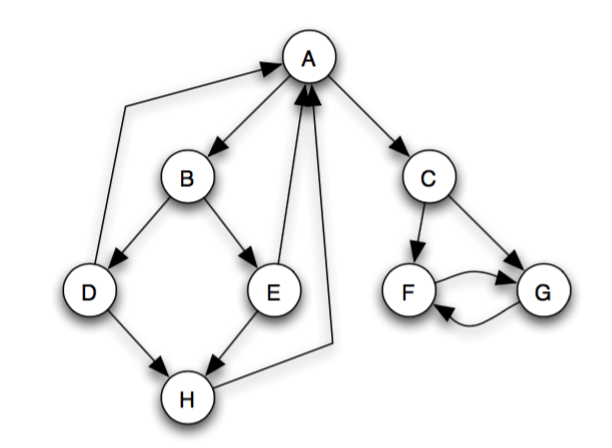
\includegraphics[scale=0.2]{img/wrong_nodes.png} 
\end{center}
The Wrong nodes are a small sets of nodes that can be reached from the rest of the graph, but have no paths back.
\end{frame}

\begin{frame}
\frametitle{Scaled PageRank }
We can use the mechanism of fluid presented before: there is a \alert{counter-balancing process} preventing that all the water stands only on downhill places on the earth.
\begin{block}{Scaled PageRank Update Rule}
First apply the Basic PageRank Update Rule.\\ 
\smallskip
Then scale down all PageRank values by a factor of s, shrinking the total from 1 to s. \\
\smallskip
We divide the residual $1 - s$ units of PageRank equally over all nodes, giving$ (1 - s)$/$n$ to each.
\end{block}
\end{frame}

\begin{frame}
\frametitle{Results}
We are going to present the result of the experiment, comparing the \alert{execution time} of PageRank on following inputs:
\begin{itemize}
\item Graph of 1000 nodes
\item Graph of 2000 nodes
\item Graph of 5000 nodes
\item Graph of 10000 nodes
\item Graph of 20000 nodes
\item Full Graph (30000 nodes) 
\end{itemize}
All the graphs are generated by chunking the Full Graph.
\end{frame}

\begin{frame}
\frametitle{Graph of Times}
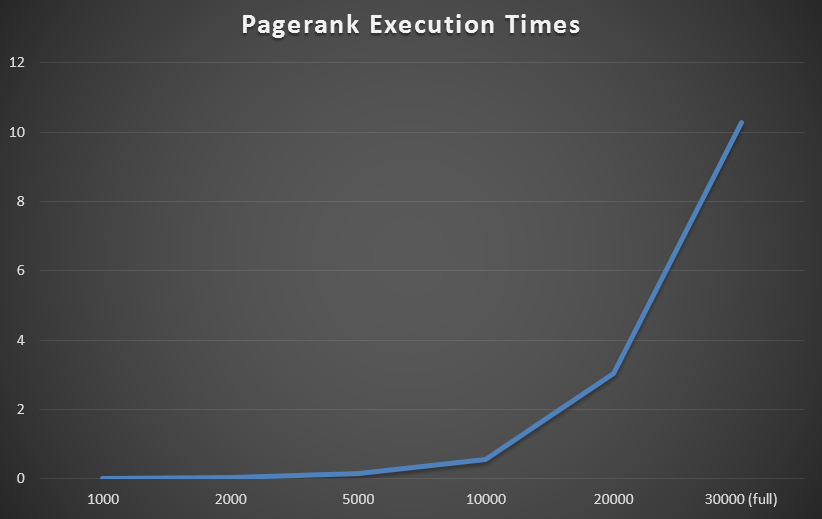
\includegraphics[scale=0.5]{img/Ranking/Pagerank.PNG} 
\end{frame}

\subsection{HITS}
\begin{frame}
\frametitle{HITS}
This hubs-and-authorities algorithm, sometimes called HITS (\textit{hyperlinkinduced
topic search}), was originally intended not as a preprocessing step before
handling search queries, as PageRank is, but as a step to be done along with
the processing of a search query, to rank only the responses to that query.\\
\medskip
This kind of approach is  used by the Ask search engine.
\end{frame}

\begin{frame}
\frametitle{The Intuition Behind HITS}
HITS views important page as having two different type of importance.
\begin{itemize}
\item Certain pages are valuable because they provide information about a
topic. These pages are called \textbf{authorities}.
\item Other pages are valuable not because they provide information about any
topic, but because they tell you where to go to find out about that topic.
These pages are called \textbf{hubs}.
\end{itemize}
\end{frame}

\begin{frame}
\frametitle{HITS Algorithm}
For calculate the HITS values for the pages, we shall assign two scores to each Web page.
One score represents the \textit{hubbiness} of a page  that is, the degree to which it
is a good hub, and the second score represents the degree to which the page
is a good authority.\\
\medskip
These values  are then calculated as:
\begin{itemize}
\item \onslide<1-> \textbf{Hubbiness}: the sum of the Authority value of the outgoing nodes.
\item \onslide<2-> \textbf{Authority}: the sum of Hubbines value of the incoming nodes.
\end{itemize}
\-\\\
\smallskip
\onslide<3-> These values are normalized that the largest value is 1.
\end{frame}

\begin{frame}
\frametitle{Results}
We are going to present the result of the experiment, comparing the \alert{execution time} of HITS on following inputs:
\begin{itemize}
\item Graph of 1000 nodes
\item Graph of 2000 nodes
\item Graph of 5000 nodes
\item Graph of 10000 nodes
\item Graph of 20000 nodes
\item Full Graph (30000 nodes) 
\end{itemize}
All the graphs are generated by chunking the Full Graph.
\end{frame}

\begin{frame}
\frametitle{Graph of Times}
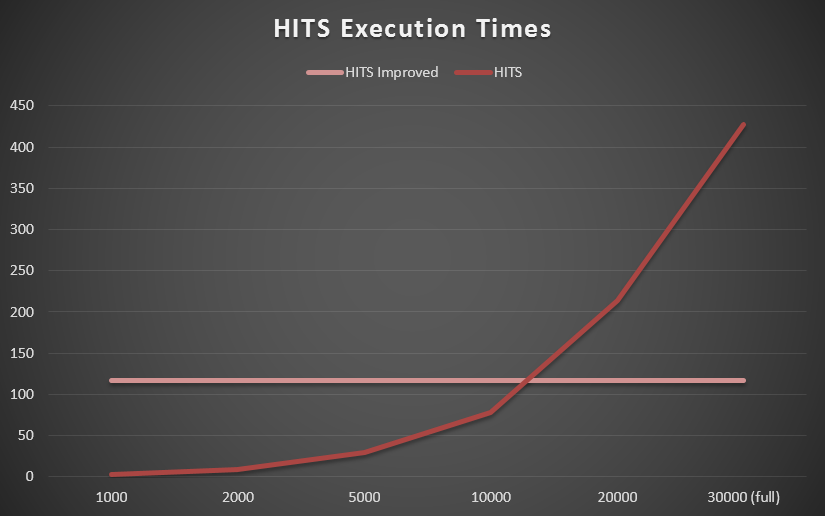
\includegraphics[scale=0.5]{img/Ranking/HITS.PNG} 
\end{frame}

\begin{frame}
\frametitle{Tuning for improving performance}
On the first attempts of running the algorithm on the full graph we observed that one iteration takes about 30 minutes, this is due to the nature of the algorithm. \\
In each iteration we explore all the graph and calculate the incoming node for the current node \dots\\
\bigskip
Considering that graph never changes, we precomputed all the incoming nodes for each node so we can obtain the incoming nodes in $O(1)$.
\end{frame}

\begin{frame}
\frametitle{Tuning for improving performance}
In the HITS algorithm there are two stop rules:
\begin{itemize}
\item Max number of iteration
\item Min confidence on the errors reached
\end{itemize}
\medskip
But we denote in some case that the Algorithm runs until max number of steps are reached, and when this happen the relative error tent to stabilize on a level remain fixed on that, so we added a new stop rule: \\
\medskip
\begin{itemize}
\item If the the two successive relative errors are equals more a small $\epsilon$ then stop the algorithm.
\end{itemize}
\end{frame}

\subsection{Comparing the Results}
\begin{frame}

\end{frame}

\section{Matching}
\subsection{Best Match}
\begin{frame}

\end{frame}

\subsection{Improved Best Match}
\begin{frame}

\end{frame}

\subsection{Results}
\begin{frame}

\end{frame}

\section{Search Engine}
\begin{frame}

\end{frame}

\section{Auction}

\subsection{First Price Auction}
\begin{frame}

\end{frame}

\subsection{Generalized Second Price Auction}
\begin{frame}

\end{frame}

\subsection{Results}
\begin{frame}

\end{frame}



\end{document}